\chapter*{Úvod}
\label{UVOD}
\addcontentsline{toc}{chapter}{Úvod}

Cieľom tejto práce je návrh, výroba a naprogramovanie modernej učebnej pomôcky AeroShieldu (ďalej len „shield”), ktorá slúži na výučbu základov teórie riadenia a elektrotechniky. Učebné pomôcky sú nevyhnutnou, no často zanedbávanou súčasťou výučby. Študenti si vďaka nim môžu lepšie predstaviť a pochopiť problematiku daného učiva, keďže môžu pracovať nie len s počítačovými modelmi sústavy, ale aj s jej fyzickou reprezentáciou. Avšak, takéto pomôcky bývajú častokrát príliš zložité na používanie a priveľmi drahé \cite{Hor}. Z týchto dôvodov je ich použitie pri výučbe častokrát nepraktické.
 
Experimentálny modul vzdušného kyvadla je pomerne jednoduché zariadenie, pozostávajúce z niekoľkých častí. Akčným členom kyvadla je motorček, ktorý má na rotor pripojené lopatky, ktoré vďaka otáčaniu produkujú ťah. Motorček je zvyčajne upevnený na koniec ľahkej tyčky, ktorá je v mieste otáčania pripevnená k zariadeniu na meranie uhlu pootočenia. Zariadenie na meranie pootočenia môže byť potenciometer, senzor hallovho javu(efektu), alebo iné \cite{senzor}. Zariadenie na meranie uhlu je následne upevnené na podstavec, ktorý zariadenie stabilizuje a umožňuje volný pohyb kyvadla. 
 
Tvorba AeroShieldu bola inšpirovaná experimentom známym pod názvom Aeropendulum, čo v doslovnom preklade znamená vzdušné kyvadlo. Na túto tému existuje niekoľko odborných článkov, ktoré sa zaoberajú zostavením, ovládaním, alebo simuláciami takéhoto kyvadla. Medzi najviac citované články patria práce autorov Mila Mary Job a P. Subha Hency Jose\cite{7192959} a dvojice Eniko T. Enikov a Giampiero Campa\cite{enikov_campa_2012}. Práca Mila Mary Job a P. Subha Hency Jose bola zameraná hlavne na simuláciu kyvadla a matematiku, ktorá je na takúto simuláciu potrebná. Kyvadlo od autorov Eniko T. Enikov a Giampiero Campa vznikalo na univerzite Arizona. Ovládané bolo pomocou špeciálne navrhnutej dosky plošných spojov a ktorá sa programovala v softvéri Simulink. 

Na Arizonský projekt nadviazali aj dve záverečné práce vypracované na Strojníckej fakulte Slovenskej technickej univerzity v Bratislave. Boli to diplomové práce študentov Andreja Poláka\cite{Polak} a Jakuba Onderu\cite{Ondera}. Tieto práce sa zaoberali vylepšením Arizonského kyvadla, lepším pohonom, presnejším ovládaním, rôznymi meraniami polohy a zrýchlenia a zmenou ovládacieho modulu za mikrokontrolér Arduino. Cena tohoto kyvadla bola vzhľadom na použité materiály a množstvo súčiastok pomerne vysoká, rádovo stovky eur. 

Existuje niekoľko spoločností, ktoré na predaj ponúkajú hotové experimentálne moduly vzdušného kyvadla. Konkrétne sa jedná napríklad o kyvadlo značky Real Sim obr.\ref{OBRAZOK 1.2}.a, ktorá ponúka hotový, zostavený modul. Cenu tohoto kyvadla sa nám žiaľ nepodarilo dohľadať. Ďalším takýmto modulom je kyvadlo od univerzity Arizona\cite{enikov_campa_2012} obr.\ref{OBRAZOK 1.2}.b, ktoré je predávané ako nezostavený model. Cena tohoto kyvadla je 95\euro. 

\begin{figure}[!tbh]
	\hfill
	\subfigure[{Aeropendulum značky Real Sim\cite{AeroPendulumTeheran}.}]{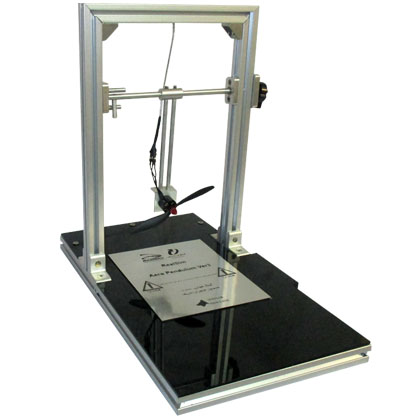
\includegraphics[width=8cm]{obr/pendulum.jpg}}
	\hfill
	\subfigure[{Aeropendulum univerzity Arizona\cite{enikov_campa_2012}.}]{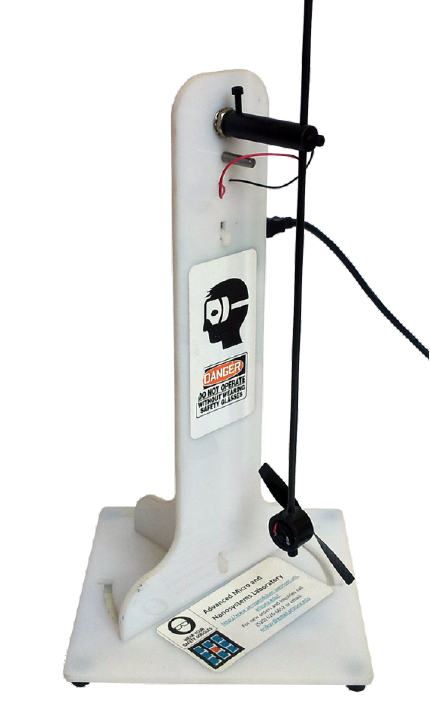
\includegraphics[width=6.5cm]{obr/arizona.png}}
	\hfill
	\caption{Experimentálne moduly vzdušného kyvadla.}\label{OBRAZOK 1.2}
\end{figure}

\newpage
Open-source\footnote[1]{Open-source je zo všeobecného pohľadu akákoľvek informácia, ktorá je dostupná verejnosti bez poplatku(s voľným prístupom), s ohľadom na fakt, že jej voľné šírenie zostane zachované.} projekt AutomationShield je zameraný na vývoj hardwarových a softwarových nástrojov určených na vzdelávanie a doplnenie vzdelávacieho procesu. Jadrom celého projektu je tvorba rozširujúcich dosiek (shieldov) vyvíjaných pre populárny typ prototypizačných dosiek s mikrokontrolérmi Arduino. Tieto pomerne lacné učebné pomôcky, majú za cieľ lepšiu výučbu strojného inžinierstva, mechatroniky a základov automatického riadenia\cite{Auto}.

Všetky informácie ohľadom projektu AutomationShield, sú dostupné na platforme GitHub\cite{Git}, ktorá slúži ako knižnica kódov, návodov a postupov, ktoré sú voľne dostupné na čítanie a úpravu. Na samostatnej stránke AutomationShieldu nájdeme zoznam jednotlivých shieldov a to, v akom procese výroby a fungovania sa nachádzajú. Ku každému shieldu nájdeme jeho podrobnú dokumentáciu, knižnice, zdrojové kódy, ako aj predprogramované ukážky jeho fungovania. GitHub je open-source platforma. Dokumenty zdieľané na tejto stránke teda môže ktokoľvek upravovať, kontrolovať alebo vylepšovať, čo tvorí ideálny priestor pre rozvoj nových myšlienok a podporu tvorivého procesu.

\newpage
Hlavnou motiváciou tohoto projektu je nízka dostupnosť a vysoká cena podobných učebných pomôcok. Z môjho pohľadu je výučba častokrát až príliš zameraná na memorovanie faktov a teórie, namiesto praktických experimentov a skúseností typu pokus-omyl. Študenti pochopia vyučovanú teóriu jednoduchšie, pokiaľ majú možnosť experimenty sami tvoriť, skúmať a testovať\cite{Dhanapal2013ASO}. 

S úmyslom priniesť širokej verejnosti lacnejšiu a výkonnejšiu alternatívu vtedajším mnohonásobne drahším a menej výkonným prototypizačným doskám\cite{stamp} prišla na trh v roku 2005 prototypizačná doska Arduino. Projekt vznikol v Taliansku ako kolaborácia medzi viacerými nadšencami elektrotechniky a programovania, na ktorého čele bol Massimo Banzi. Veľkou výhodou dosiek Arduino a ich nadstavbových shieldov je fakt, že sú pomerne lacné a majú malé rozmery (Arduino UNO: 68.6*53.4mm\cite{UNO}). Tieto skutočnosti umožňujú študentom pracovať na experimentoch nielen na pôde školy, ale experimenty si môžu zobrať domov a pracovať na nich aj mimo vyučovacieho procesu. 

\begin{figure}[!tbh]
	\centering
	\includegraphics[width=80mm]{obr/arduino.jpg}
	\caption{{Arduino UNO R3.\cite{UNOFOTO}}}\label{OBRAZOK 1.3}
\end{figure}

Na fungovanie a programovanie dosky postačuje len USB kábel, programovací softvér a samotná doska. Vzhľadom na nízky počet potrebných súčiastok a fakt, že mikročip Arduina je v prípade poruchy jednoducho vymeniteľný\footnote[2]{Platí pri mikročipoch typu DIP(Dual in-line package), ktoré stačí jednoducho vytiahnuť z konektora bez použitia spájkovania.}, je jeho používanie na školách príjemné a jednoduché. Mikrokontroléri Arduino využívame z dôvodu nízkej ceny, širokej dostupnosti rôznych modelov, postačujúcej výpočtovej sile a príjemnému používateľskému rozhraniu. Pre naše účely využívame dve verzie Arduina. Prvou z nich je doska Arduino UNO R3  obr.\ref{OBRAZOK 1.3}, ktorú používame na programy Arduino API. Na doske sa nachádza 14 digitálnych a 6 analógových pinov.

Na prácu v MATLABE a Simulinku využívame Arduino Mega 2560 R3 obr.\ref{OBRAZOK 1.32}. Na tejto doske sa nachádza 54 digitálnych a 16 analógových pinov. AeroShield je kompatibilný so všetkými doskami s označením R3, alebo s doskami ktoré majú rozloženie pinov rovnaké ako Arduino UNO R3. 

Niektoré piny sú označené špeciálnym symbolom $"$$\sim$$"$. Tieto piny sú schopné generovať PWM\footnote[3]{Šírková modulácia impulzov alebo PWM je technika na dosiahnutie analógových výsledkov pomocou digitálnych prostriedkov a to za pomoci striedania dĺžok medzi High a Low stavom, resp. zapnutý a vypnutý stav.} signál, ktorý využívame na ovládanie motora kyvadla.

\begin{figure}[!tbh]
	\centering
	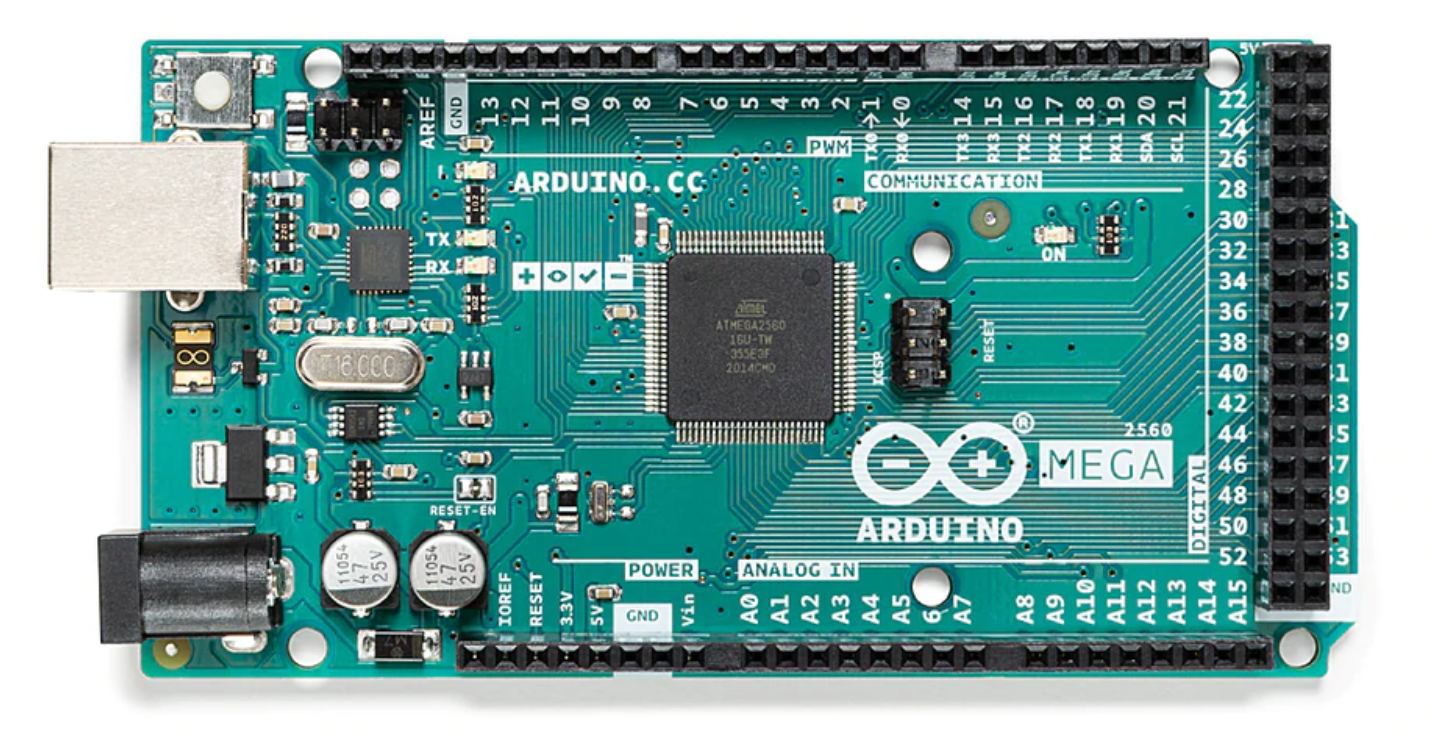
\includegraphics[width=100mm]{obr/mega.png}
	\caption{{Arduino Mega 2560 R3.\cite{megafoto}}}\label{OBRAZOK 1.32}
\end{figure}

\newpage
Práca je rozdelená do štyroch logických celkov. Na začiatku v časti Hardvér je opísaný základný princíp fungovania shieldu a následne jeho jednotlivé súčiastky. Nasleduje časť tvorby schémy zapojenia shieldu a dosky plošných spojov v programe DipTrace. Na konci časti Hardvér je spomenutá tvorba modelu kyvadla a cenová kalkulácia výroby experimentálneho modulu. 

V softvérovej časti sú bližšie predstavené spôsoby programovania shieldu. Opisuje sa tu tvorba knižníc jednotlivých programov, v ktorých sú tvorené didaktické príklady pre AeroShield.

Poslednú časť práce tvoria samotné didaktické príklady nasledované finálnym zhodnotením práce.




